Esse capítulo tem como objetivo mostrar a metodologia utilizada para atingir o objetivo do trabalho. A Figura \ref{figure:metodologia} mostra, de maneira geral, o esquema da metodologia proposta. Primeiramente, será discutido o ambiente de experimento. Em seguida, será explicitado como os dados foram pré-processados. Por último, será discutido a escolha e implementação dos modelos e as métricas de avaliação utilizadas, assim como qual foi o ambiente de teste utilizado.

\begin{figure}
    \centering
    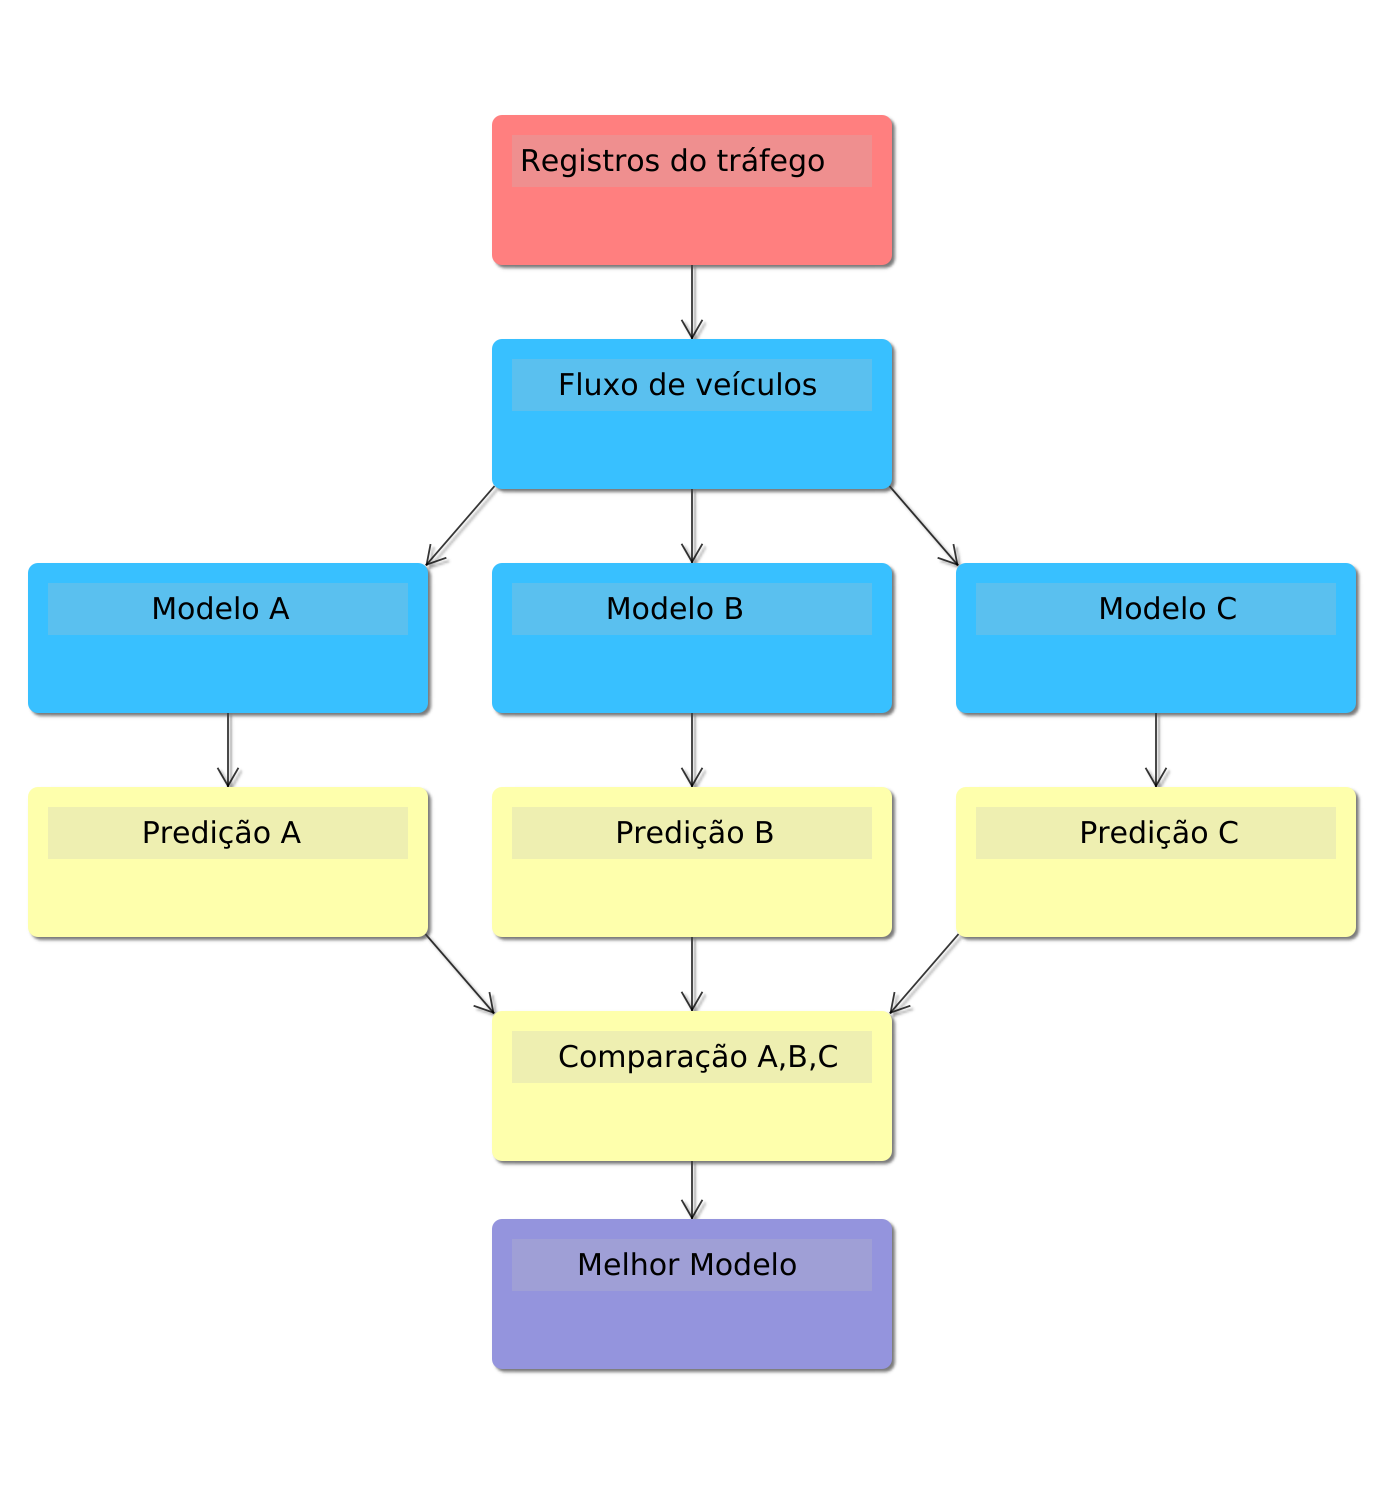
\includegraphics[scale=0.4]{monography/img/tccFlux.png}
    \label{figure:metodologia}
    \caption[Fluxograma da metodologia]{Fluxograma da metodologia}
\end{figure}

\section{Ambiente de Experimento}

O ambiente de experimento foi um servidor equipado com Ubuntu 64 bits. O servidor possui dois CPUs \textit{Intel(R) Xeon(R) Platinum 8160 CPU @ 2.10GHz} e 251 GiB de memória principal. Cada CPU dessas possui 24 núcleos e executa até 48 \textit{threads} em paralelo. No total então são 96 \textit{threads}, que foram usados paralelamente para acelerar a execução do experimento. Porém, em algumas partes da execução, menos \textit{threads} tiveram que ser usadas, pois não havia memória principal o suficiente para todas as instâncias em paralelo.

\section{Pré-Processamento dos Dados}

Nesta etapa serão feitos ajustes no conjunto de dados inicial, como remoções de inconsistências e transformações nos dados mostrados na Tabela \ref{table:data}. Esse ajustes têm como propósito melhorar a aprendizagem dos modelos que serão utilizados. Subsequentemente, será mostrado como os conjuntos de treino e teste foram criados a partir do conjunto de dados e das variações do modelo. Por fim, é realizado uma exploração da sazonalidade do fluxo.

\subsection{Limpeza dos Dados}

No conjunto de dados inicial existem colunas que não são relevantes para o problema, ou possuem algum tipo de inconsistência. Devido a este fato, as colunas a seguir serão removidas:

\begin{itemize}
    \item \texttt{Faixa}
    \item  \texttt{Hora}
    \item \texttt{Limite de Velocidade da Via}
    \item  \texttt{Tamanho do Veículo}
\end{itemize}

A coluna \texttt{Faixa} será removida, pois nas transformações que virão a seguir, esse dado se tornará desnecessário, visto que o objetivo deste trabalho é prever o fluxo na via como um todo e não em faixas específicas. A coluna \texttt{Hora} será removida, pois com o intervalo de fluxo, já é possível saber a qual momento do dia se refere determinado registro. Além disso, para utilizar a hora propriamente dita como entrada dos modelos, seria necessária uma análise mais minuciosa de como tratá-la, o que foge do escopo definido pelo trabalho. A coluna \texttt{Limite de Velocidade da Via} será removida, pois este dado tem seu valor repetido ao longo de todos os registros, isto é, o valor é constante em todo o conjunto de dados e não afeta no treinamento dos modelos. A coluna \texttt{Tamanho do Veículo} será removida, pois não foi medida de forma precisa, visto que existem registros com veículos de tamanho zero (o que não é fisicamente possível).

\subsection{Transformação dos Dados}

A transformação dos dados se torna útil quando um tipo de dado pode ser representado de outra forma, em geral mais simples, que ajude no treinamento do modelo. No caso, a coluna \texttt{Data} será transformada, pois existem diversas informações subtendidas em uma data como dia da semana, se é feriado, início ou fim do mês, entre outros. Essas informações que podem ser extraídas de uma data podem ter uma relação direta ou indireta com o comportamento de uma via. Visto que a quantidade de dados que temos não chega nem a cobrir todas as datas de 1 ano, se torna difícil para os modelos aprenderem a extrair e utilizar essas informações. 

Sendo assim, a coluna \texttt{Data} será simplificada para o dia da semana, dado que o fluxo aparenta apresentar comportamentos similares nos mesmos dias da semana. Para evitar falsas suposições do modelo, será utilizado a técnica \textit{one hot encoding} para transformar essa coluna \texttt{Data} e 7 colunas diferentes (uma para cada dia da semana). Cada uma dessas colunas terá valores 1 ou 0 para representar se é ou não um certo dia da semana. Isso é necessário, pois caso fosse uma coluna quantitativa (0 representando domingo e 1 representando segunda, por exemplo) o modelo poderia realizar inferências, como ``segunda'' é maior que ``quarta'', ou analogias similares.

\subsection{Acumulação dos registros}

Como visto na literatura, existem algumas maneiras diferentes de se fazer a predição de veículos em uma via. Seja pelo fluxo, pela densidade, ou pela velocidade média dos veículos. Neste trabalho, optou-se por utilizar o fluxo como método de predição, seguindo o padrão visto em \cite{lana_2018}. Para o cálculo do fluxo deste trabalho, foi utilizado o sensor \textbf{RSI128} disponível no conjunto de registros iniciais.

Sendo assim, o conjunto de dados será transformado de uma série temporal de registros de veículos para uma série temporal de fluxos. Isto é, será calculado a quantidade de veículos que passaram por um local em um determinado intervalo de tempo. Além disso, também foram calculadas a velocidade média e a densidade no mesmo intervalo. Para definir o intervalo que foi utilizado, testou-se os valores de intervalo para 2.5, 5 e 7.5 minutos. Note que foram utilizados intervalos que sejam múltiplos de 15, visto que todos os tempos de predição no futuro serão múltiplos de 15.

É preciso levar em consideração que quando se acumula os registros em um intervalo de tempo muito pequeno, o conjunto de dados apresenta muito ruído, dificultando a aprendizagem e afetando a qualidade da previsão. Em contrapartida, ao se aumentar o intervalo, o conjunto de dados pode se tornar muito pequeno, o que também pode dificultar a aprendizagem. Para se escolher qual dos intervalos seria o melhor para a predição, o tamanho do intervalo de fluxo será um dos parâmetros a serem escolhidos. Isto é, será realizado uma comparação entre os modelos para ver como que eles reagem. 

\begin{table}[H]
    \begin{tabular}{cccccccccc}
    \toprule
    \multicolumn{1}{l}{\textbf{Fluxo}} & \multicolumn{1}{l}{\textbf{Densidade}} & \multicolumn{1}{l}{\textbf{Velocidade Média}} & \multicolumn{1}{l}{\textbf{Dom}} &
    \multicolumn{1}{l}{\textbf{Seg}} & \multicolumn{1}{l}{\textbf{Ter}} & \multicolumn{1}{l}{\textbf{Qua}} & \multicolumn{1}{l}{\textbf{Qui}} &
    \multicolumn{1}{l}{\textbf{Sex}} &
    \multicolumn{1}{l}{\textbf{Sab}} \\
    \midrule
     6 & 0.260870 & 23.500000 & 0 & 0 & 0 & 0 & 0 & 0 & 1 \\
    \midrule
    17 & 0.586207 & 29.235294 & 0 & 0 & 0 & 0 & 0 & 0 & 1 \\
    \midrule
    15 & 0.625000 & 24.933333 & 0 & 0 & 0 & 0 & 0 & 0 & 1 \\
    \midrule
    18 & 0.666667 & 27.500000 & 0 & 0 & 0 & 0 & 0 & 0 & 1 \\
    \midrule
    14 & 0.736842 & 19.500000 & 0 & 0 & 0 & 0 & 0 & 0 & 1 \\
    \midrule
    14 & 0.700000 & 20.571429 & 0 & 0 & 0 & 0 & 0 & 0 & 1 \\
    \midrule
     6 & 0.352941 & 17.833333 & 0 & 0 & 0 & 0 & 0 & 0 & 1 \\
    \midrule
     8 & 0.400000 & 20.375000 & 0 & 0 & 0 & 0 & 0 & 0 & 1 \\
    \midrule
    11 & 0.550000 & 20.181818 & 0 & 0 & 0 & 0 & 0 & 0 & 1 \\
    \midrule
    15 & 0.652174 & 23.466667 & 0 & 0 & 0 & 0 & 0 & 0 & 1 \\
    \midrule
    10 & 0.588235 & 17.700000 & 0 & 0 & 0 & 0 & 0 & 0 & 1 \\
    \midrule
    13 & 0.722222 & 18.769231 & 0 & 0 & 0 & 0 & 0 & 0 & 1 \\
    \midrule
    11 & 0.785714 & 14.363636 & 0 & 0 & 0 & 0 & 0 & 0 & 1 \\
    \midrule
     8 & 0.400000 & 20.125000 & 0 & 0 & 0 & 0 & 0 & 0 & 1 \\
    \midrule
     8 & 0.347826 & 23.750000 & 0 & 0 & 0 & 0 & 0 & 0 & 1 \\
    \bottomrule
    \end{tabular}
    \label{table:data_pre}
    \caption{Amostra do pré-processamento dos dados ao se utilizar 7.5 minutos de intervalo do sensor RSI128}
\end{table}

No final do pré-processamento o resultado possuirá 3 colunas quantitativas e 7 qualitativas. As colunas de \textit{Densidade} e \textit{Velocidade Média} são contínuas e a coluna \textit{Fluxo} é discreta. As outras 7 colunas representam uma classificação indicando se é ou não (0 representa falso e 1 verdadeiro) um certo dia da semana, sendo assim uma coluna qualitativa ordinal.

Vale notar que, como o período é o mesmo para qualquer um dos sensores, ao se acumular os registros, o tamanho do conjunto de dados será sempre igual. Isto é, será equivalente ao intervalo de tempo do conjunto de dados, 92 dias, divido pelo tempo de agregação de fluxo (7.5 minutos), o que gera 17.664 registros de fluxo dos 536.879 registros de passagem de veículos disponíveis.

\subsection{Normalização dos Dados}

Na área de aprendizagem de máquina, é comum vermos modelos de predições para diferentes tipo de variáveis. Por vezes, os valores assumidos por essas variáveis podem apresentar um domínio grande demais, como no caso da predição de valores de ações da bolsa de valores. Com valores em um intervalo tão grande, o treinamento dos modelos tende a piorar. Para contornar este problema, é comum utilizar técnicas que visam diminuir o intervalo de valores que as variáveis podem assumir. Uma destas técnicas é a normalização. 

Em um dos tipos da normalização, utiliza-se o maior e o menor valor que o seu conjunto de dados atinge para ajustar os valores intermediários, como pode ser visto em \cite{Dorian_1999}. Por exemplo, o maior fluxo calculado foi 94 veículos para o sensor \textbf{RSI128} com acumulação de 2,5 minutos e o menor foi 0. Assim, foram ajustados os valores do conjunto de dados dentro de um intervalo entre 0 e 1, com 0 representando o menor valor e 94, o maior valor. Porém, os testes realizados mostraram que a normalização não trouxe melhorias significativas para as predições deste trabalho, apresentando, inclusive, resultados levemente piores em alguns modelos. Por este motivo, optou-se por continuar os experimentos sem normalização.

\subsection{Criação dos Conjunto de Treino e Teste}

Será utilizado o conjunto dos dados pré-processados (\(D\)) para gerar o conjunto de dados de treino (\(X\)) e teste (\(Y\)). Cada elemento (\(x_i\)) do conjunto de treino  será uma série temporal dos atributos. Essa série temporal representa uma visão contínua do passado em relação ao presente momento. Ou seja, cada elemento de treino será uma subsequência de \(D\) de tamanho \(m\), onde cada instância (\(x_{i, j}\)) é uma das linhas da Tabela \ref{table:data_pre}. Para o conjunto de testes, cada elemento (\(y_i\)) será o fluxo no futuro (\(x_{i + k, m_{fluxo}}\)). Para fins de análise, será utilizado o conjunto de treino para gerar um outro conjunto mais simples. Este novo conjunto possuirá apenas o fluxo. Desta forma, será possível comparar os resultados dos modelos utilizando apenas o fluxo com os resultados dos modelos utilizando a densidade e a velocidade média também. Com isso, será possível dizer se as colunas de \texttt{Velocidade Média}, \texttt{Densidade} e as de dias da semana melhoram a performance das predições, ou não. 

No entanto, os modelos não possuem o mesmo formato de entrada de dados. Logo, é necessário adaptar o conjunto de testes aos modelos e seus formatos. Uma versão será para os modelos de aprendizagem profunda (\textit{\acrshort{LSTM}} e \textit{\acrshort{GRU}}) com três dimensões (amostras por sequência por atributos), assim como mostrado acima. A outra versão será para os modelos tradicionais (\textit{\acrshort{RF}} e \textit{\acrshort{SVM}}), que terá somente duas dimensões (amostras por atributos). Ou seja, \(x'_i\), nesse caso, não é uma lista de tupla e sim somente uma tupla com todos os elementos da lista de tupla.

\subsection{Sazonalidade dos dados}

Na Figura \ref{figure:flow_discution} é mostrado o resultado da agregação dos registros de veículos em um intervalo de 7.5 minutos. É possível observar que existem flutuações na quantidade de fluxo de veículo de acordo com o dia. Este fato fica mais evidente se observarmos o primeiro pico do gráfico, referente ao Domingo, pois este apresenta um menor fluxo de veículos, o que é esperado que aconteça em um dia não comercial. Isso mostra que os dados apresentam certa sazonalidade. Esta sazonalidade se manifesta em várias escalas, no gráfico mostrado é possível ver apenas a sazonalidade referente aos dias da semana, mas ela também se aplica, por exemplo, a semana do mês, ao mês do ano, etc. 


\begin{figure}[H]
    \centering
    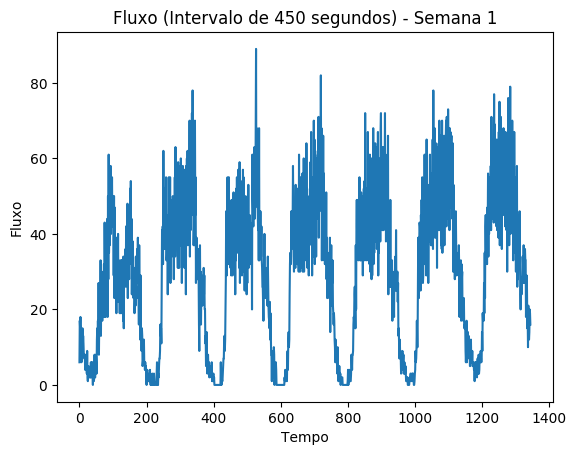
\includegraphics[scale=1]{monography/img/flows/flow_450_week_01.png}
    \label{figure:flow_discution}
    \caption[Fluxo da Primeira Semana]{Fluxo da Primeira Semana}
\end{figure}

\section{Avaliação Final}

Na literatura é comum serem utilizados as métricas \textit{\acrfull{RMSE}} e \textit{\acrfull{MAPE}} \cite{lana_2018}. Porém, como pode ser visto na Equação \ref{eq:mape}, \textit{\acrshort{MAPE}} possui divisão pelo \({y_i}\) e este pode ser zero para nosso conjunto de dados. Logo, \textit{\acrshort{MAPE}} foi descartado. 

\begin{equation}
\label{eq:mape}
MAPE = \frac{100\%}{n} \times \sum_{i=1}^{n} \quad \abs{\frac{y_i - \hat{y_i}}{y_i}}
\end{equation}

Para substituir o \textit{\acrshort{MAPE}}, será utilizado o \textit{\acrfull{MAE}}. Sendo assim, as métricas de erro dos modelos são \textit{\acrshort{MAE}} (Equação \ref{eq:mae}) e \textit{\acrshort{RMSE}} (Equação \ref{eq:rmse}).

\begin{equation}
\label{eq:mae}
MAE = \frac{1}{n} \times \sum_{i=1}^{n} \quad \abs{y_i - \hat{y_i}}
\end{equation}

\begin{equation}
\label{eq:rmse}
RMSE = \sqrt{ \frac{1}{n} \times \sum_{i=1}^{n} \quad (y_i - \hat{y_i}) ^ 2}
\end{equation}

Adicionalmente, os modelos também serão avaliados quanto a sua capacidade de acertar se o fluxo vai aumentar, ou diminuir em dado momento (15, 30, 45 e 60 minutos no futuro). Esta é uma métrica proposta por este trabalho e que não é comumente utilizada na literatura de predição de tráfego. Sua definição pode ser vista abaixo:

\begin{equation}
f(a, b, k) =
\begin{cases}
  0, & \text{if}\ (a - k) \times (b - k) \textless 0 \\
  1, & \text{otherwise}
\end{cases}
\end{equation}

\begin{equation}
\alpha = \frac{100\%}{n} \times \sum_{i=1}^{n} f(y_i, \hat{y_i}, x_{i, m_{fluxo}})
\end{equation}

\section{Out Of Sample Testing}

Para validar a performance de um modelo, é necessário fazer a utilização de métodos que comprovem a capacidade do mesmo de generalizar. Isto é, é preciso mostrar que o modelo é eficaz de maneira geral, ou para mais de um conjunto de dados. Uma das técnicas mais utilizadas é a \textit{Cross Validation}, que consiste em separar o conjunto de dados em conjuntos de dados menores para que se tenha mais blocos de dados para teste, treinamento e validação. Ao realizar esta divisão, utilizando-se \textit{Cross Validation}, a ordem dos dados não é necessariamente respeitada. Porém, o conjunto de dados deste trabalho é uma série temporal e a ordem dos registros importa, o que impossibilita a utilização deste método para este conjunto de dados. 

Entretanto, existem técnicas que se aplicam a predição de dados temporais. Tahsman et. al. \cite{Tashman_2000} e Vitor et. al. \cite{Vitor_2019} discorrem sobre esses métodos, chamados de \textit{Out of Sample Testing}, mostrando como são implementados estes tipos de validação e porque elas são adequadas para predição de séries temporais. Resumidamente, \textit{Out of Sample Testing} consiste em separar o conjunto de dados em conjunto de dados menores e independentes entre si, ou seja, dados que foram usados como treinamento em um conjunto, não serão utilizados como teste nos outros. Além de serem independentes, \textit{Out of Sample Testing} também respeita a ordem temporal dos dados, o que não afeta a correlação das informações com o tempo. Ainda em \cite{Tashman_2000}, são mostrados dois tipos de \textit{Out of Sample Testing}:

\begin{itemize}
    \item \textit{Fixed Origin}: Que consiste na definição de um, ou mais conjunto de dados derivados do conjunto de dados original, onde o ponto de divisão dos dados entre treinamento e teste é fixo.
    \item \textit{Rolling-origin}: Que consiste na definição de um, ou mais conjunto de dados derivados do conjunto de dados original, porém, neste caso, o ponto de divisão entre treinamento e teste é atualizado a cada iteração.
\end{itemize}

Neste trabalho, utilizou-se um método de \textit{Out Of Sample Testing} do tipo \textit{Rolling-Origin} chamado de \textit{Blocking}. Neste método, o conjunto de dados é dividido em subconjuntos de tamanhos iguais. Dentro de cada subconjunto, é definido o tamanho dos dados que serão utilizados para treinamento e teste.

\begin{figure}[htbp]
    \centering
    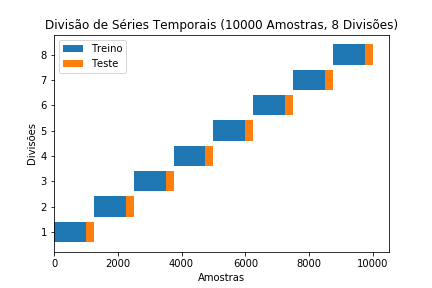
\includegraphics[scale=0.9]{monography/img/methods/blocking_cv.png}
    \label{figure:blocking}
    \caption[Representação do \textit{Out-of-Sample Testing} realizado]{Representação do \textit{Out-of-Sample Testing} realizado}
\end{figure}

\section{Modelos Desenvolvidos}

Visto que a predição do fluxo é o foco do trabalho, que temos um conjunto de pares entrada e saída e que o fluxo é quantitativo, serão utilizadas técnicas de aprendizagem de máquina supervisionadas de regressão para prever a curto prazo o fluxo da via. Quanto a essas técnicas, podemos dividi-las novamente em paramétricas e não-paramétricas.

Dos modelos não-paramétricos, se destacam o \textit{\acrfull{LSTM}} e o \textit{\acrfull{GRU}}, sendo ambos \textit{\acrshort{RNN}}'s. Quanto ao \textit{\acrfull{LSTM}}, vale ressaltar que existem diversas variações e implementações. Porém, segundo Greff et. al. \cite{Greff_2015} as variações da \textit{\acrshort{LSTM}} não possuem tantas diferenças quanto a qualidade de suas previsões. Por este motivo, este trabalho utilizou o \textit{\acrfull{LSTM}} comum. Dos modelos paramétricos, o mais utilizado na literatura para previsão de fluxo é o \textit{\acrfull{ARIMA}} e suas variações \cite{doi:10.1080/01441647.2014.992496}, além de modelos mais simples como \textit{\acrfull{LR}}. 

Todos os modelos não-paramétricos citados foram implementados para este trabalho. Quanto aos modelos paramétricos, foram testados dois modelos, sendo eles o \textit{\acrshort{ARIMA}} e o \textit{\acrshort{LR}}. Entretanto, ambos tiveram resultados muito inferiores em relação aos modelos não-paramétricos testados. Além disso, \textit{\acrshort{ARIMA}} se mostrou extremamente custoso computacionalmente de se treinar e otimizar. Por estes dois motivos citados, os modelos paramétricos foram retirados dos experimentos.

Um ponto interessante a se notar é que os modelos considerados tradicionais possuem um viés diferente dos modelos de aprendizagem profunda. Isto é, com o \acrshort{RF}, por exemplo, temos um representante dos algoritmos que utilizam árvores de decisão para realizar suas predições. Esta abordagem é completamente diferente da abordagem dos algoritmos de aprendizagem profunda, que utilizam do conceito de tentativa e erro e aprendizagem supervisionada. Essa variedade garante que os modelos não estejam todos enviesados da mesma forma.


% TODO: A gente selecionou uma quantidade de algoritmos que tem vies diferente, RF particiona como arvore (corta o espaço), SVM particiona o espaço (carta o espaço de forma linear) e é iterativo. LSTM é iterativo (Bias tried and error approach no free lunch)

\subsection{Modelos de Comparação}

Serão utilizados também dois modelos com o único propósito de estabelecer uma base de comparação inicial para os outros modelos. Serão eles o \textit{Naive} e o \acrfull{MM}. O primeiro faz suas predições apenas escolhendo o valor de fluxo mais recente (\(x_{i, m_{fluxo}}\)) dentre os valores de fluxo recebidos como entrada. Já o segundo faz a média dos valores de fluxo recebidos na entrada. Dessa forma, é possível colocar em perspectiva o desempenho dos modelos escolhidos e avaliá-los de maneira mais consistente.

\subsection{Implementação}

As arquiteturas utilizadas neste trabalho foram implementados na linguagem \textit{Python} utilizando bibliotecas como \textit{Keras} com \textit{TensorFlow} e \textit{SKLearn}. Decidiu-se por utilizar essas bibliotecas, pois suas implementações já são robustas, otimizadas e bem testadas. Implementar todos os modelos sem o auxílio de nenhuma biblioteca seria ineficiente para objetivo dos experimentos e prono a erros. Além disso, o uso das bibliotecas facilita a reprodução dos experimentos para os interessados em avançar ou verificar este projeto.

\textit{Keras} foi utilizado para implementar os modelos de \textit{\acrshort{LSTM}} e \textit{\acrshort{GRU}} e optou-se por usar como base dessa biblioteca o \textit{TensorFlow}, visto que este é o \textit{framework} com suporte para aprendizado de máquina mais utilizado dentre os desenvolvedores, segundo um questionário feito em 2018 pelo \textit{Stack Overflow} \cite{stack_2018}. Já \textit{SKLearn} foi utilizado para implementar os modelos \acrshort{RF} e \acrshort{SVM}. Também utilizou-se a biblioteca \textit {SKLearn} para realizar uma pesquisa dos melhores parâmetros de cada modelo.

\subsection{Escolha de Parâmetros}

Tanto os modelos propostos por este trabalho, quanto o conjunto de dados utilizado, podem ser ajustados para melhorar a qualidade das previsões. Os dados, como visto anteriormente, já foram tratados e corrigidos. Agora, serão realizados testes para descobrir os valores de parâmetros que produzem as melhores predições. A forma de execução dos modelos de forma genérica pode ser vista no Pseudo-Código \ref{algo:training}.

Os parâmetros definidos para os testes são: o passado visível, o número de divisões do conjunto de dados e o tamanho do intervalo do fluxo. O passado visível determina o tamanho da entrada e o quão no passado os modelos poderão enxergar do fluxo. O número de divisões afeta o tamanho das amostras de treino e teste e o tamanho do intervalo do fluxo altera o tamanho do conjunto de dados de uma forma geral. Na literatura, a escolha de parâmetros é empírica e baseada no problema. Sendo assim, os valores que foram definidos para serem testados neste trabalho foram os seguintes:

\begin{itemize}
    \item \textbf{Número de divisões do conjunto de dados} (\textit{Blocking}): 1, 2, 4, 8 divisões;
    \item \textbf{Passado Visível}: 60, 120, 240 e 480 minutos;
    \item \textbf{Tamanho do Intervalo para cálculo do fluxo}: 150, 300, 450 segundos;
\end{itemize}

Para o número de divisões e passado visível é utilizado uma escala exponencial para que seja possível observar como essas variáveis afetam os modelos à medida que crescem. O número de divisões tem seu valor máximo definido como 8, pois um número muito maior faria com que o conjunto de treinamento tivesse menos de 1 semana. Passado visível tem seu valor máximo definido como 480 minutos por limitações de hardware. Já o tamanho do intervalo acumulado é limitado a divisores de 15 minutos, visto que o trabalho tem como objetivo prever como o fluxo estará após 15, 30, 45 e 60 minutos. Além disso, tempos de acumulação inferiores tornam o conjunto de dados muito ruidosos, ao passo que valores de acumulação muito altos tornam o conjunto de dados muito pequeno.

\subsection{Escolha de Hiper-Parâmetros}

% TODO: melhorar a escrita deste parágrafo
A escolha de hiper-parâmetros, diferente da escolha de parâmetros, é mais sensível. Isto é, os melhores hiper-parâmetros são mais sensível a mudança dependendo dos dados. Sendo assim, é uma tarefa complexa recomendar um conjunto de hiper-parâmetros que resolve o problema de previsão de fluxo a curto prazo. Com isso em mente, os modelos foram alterados para que a escolha de hiper-parâmetros fizesse parte do treino assim como mostrado no Pseudo-Código \ref{algo:tuned_training}. Como essa escolha agora faz parte do treino e são realizadas diversos treinos devido ao \textit{Out-of-Sample-Testing}, teremos várias escolhas de hiper-parâmetros e podemos verficar quais foram as mais comuns.

Como escolha de hiper-parâmetros (\textit{tuning}) será utilizada para verificar a sensibilidade dos modelos com os hiper-parâmetros antes escolhidos. Para essa fase, o conjunto de testes é novamente divido em dois(treino e teste \textit{tuning}). Esta etapa é necessária para evitar o sobre-ajuste (\textit{overfitting}) e para garantir que os resultados finais sejam genéricos o suficiente para casos nunca visto antes (outro conjunto de dados, por exemplo). Os testes realizados serão feitos de forma que todos os hiper-parâmetros sejam testados uns com os outros, ou seja, todas as combinações e instâncias possíveis serão verificadas. 

Para os modelos de aprendizagem profunda (\textit{\acrshort{LSTM}} e \textit{\acrshort{GRU}}) os hiper-parâmetros são os mesmos. Segundo Greff et. al. \cite{Greff_2015}, que realizou extensos testes nesses dois modelos, os dois fatores que mais afetam a previsão dos modelos citados são a taxa de aprendizado e o tamanho da rede. Sendo assim, esses dois foram escolhidos como os hiper-parâmetros, com as opções sendo:

\begin{itemize}
    \item \textbf{Taxa de Aprendizado}: 0.001, 0.004, 0.016 e 0.064;
    \item \textbf{Número de Células da Rede}: 50, 75, 100, 125 células;
\end{itemize}

A taxa de aprendizado tem uma escala exponencial, onde o menor valor se baseia no valor padrão escolhido pelo biblioteca \textit{Keras}. Já o número de células da rede é limitada pelo hardware, visto que se tem um crescimento computacional significativo ao se aumentar o número de células. 

Para \textit{\acrshort{RF}} os hiper-parâmetros foram escolhidos para evitar o sobre-ajuste seguindo, em parte, a sugestão de Trevor Hastie et al. \cite{hastie2005elements} para construção de árvores e variando a quantidade de estimadores. Sendo assim, os hiper-parâmetros escolhidos foram a quantidade de estimadores (árvores) e altura máxima das árvores. A quantidade de estimadores e a altura máxima das árvores foram escolhido também um escala exponencial para ver como o modelo reage a medida que os valores crescem.  Sendo os valores escolhidos:

\begin{itemize}
    \item \textbf{Quantidade de Estimadores}: 50, 100, 200, 400, 800 estimadores;
    \item \textbf{Altura Máxima}: 8, 16, 32, 64 e sem limitações no tamanho;
\end{itemize}

Para \textit{\acrshort{SVM}}, segundo Vladimir Cherkassky et. al. \cite{CHERKASSKY2004113}, a literatura não entra em consenso quanto a uma recomendação de hiper-parâmetros, com até algumas se contradizendo. Sendo assim, foram escolhidos os hiper-parâmetros C que indica quanto os erros serão penalizados e o parâmetro Os valores escolhidos foram:

\begin{itemize}
    \item \textbf{C}: 1, 10, 100 e 1000;
    \item \textbf{\(\gamma\)}: 4 valores espaçados, do espaço logarítmico de -2 a 2, e o padrão da biblioteca; 
\end{itemize}

% TODO: terminar SVM
O hiper-parâmetro C representa ... Já o hiper-parâmetro \(\gamma\) representa ...

\begin{algorithm}
\label{algo:training}
\caption{Pseudo-Código de Treinamento dos Modelos Sem \textit{Tuning}}
\begin{algorithmic}
\REQUIRE $X$, $Y$, $k$ (número de divisões)
\ENSURE $[\hat{y_0}, ..., \hat{y_k}]$
\STATE $\hat{Y} \leftarrow [] $
\newline
\FOR{$(X_{train}, X_{test}, Y_{train}, Y_{test})$ $\in$ divisaoBlocos(X, Y, k)} 
    \STATE $modelo \leftarrow geraModelo()$
    \STATE $modelo \leftarrow treinaModelo(modelo, X_{train}, Y_{train})$ 
    \newline
    \STATE $\hat{y} \leftarrow predizModelo(modelo, X_{test}) $
    \STATE $\hat{Y} \leftarrow \hat{Y} + \hat{y}$
\ENDFOR
\newline
\RETURN $\hat{Y}$
\end{algorithmic}
\end{algorithm}

\begin{algorithm}
\label{algo:tuned_training}
\caption{Pseudo-Código de Treinamento dos Modelos Com \textit{Tuning}}
\begin{algorithmic}
\REQUIRE $X$, $Y$, $k$ (número de divisões)
\ENSURE $[\hat{y_0}, ..., \hat{y_k}]$
\STATE $\hat{Y} \leftarrow [] $ 
\newline
\FOR{$(X_{train}, X_{test}, Y_{train}, Y_{test})$ $\in$ divisaoBlocos(X, Y, k)} 
    \STATE $hp \leftarrow pegarHiperParametros()$
    \STATE $dados \leftarrow divisaoBlocos(X_{train}, Y_{train}, 1)$
    \STATE $modelo \leftarrow escolheMelhorModelo(geraModelo, hp, dados)$
    \newline
    \STATE $modelo \leftarrow treinaModelo(modelo, X_{train}, Y_{train})$ 
    \newline
    \STATE $\hat{y} \leftarrow predizModelo(modelo, X_{test}) $
    \STATE $\hat{Y} \leftarrow \hat{Y} + \hat{y}$
    \newline
\ENDFOR
\newline
\RETURN $\hat{Y}$
\end{algorithmic}
\end{algorithm}